\label{sec:recurrence-transfer}

Marker 7 is the one candidate whose target is itself a downstream clinical outcome
(biochemical recurrence) rather than a molecular or morphological status. This section covers
its full story together: the prospectively frozen LEOPARD 3-pool test of whether qualification
transfers to this outcome, marker 7's own post-hoc discovery and exploratory cross-cohort evaluation, its
confounder audit against both grade alone and a fully-adjusted clinical baseline, and its
benchmarking against standard TCGA endpoints.

\subsection{LEOPARD 3-pool design}
\label{sec:leopard-methods}

Following the protocol-freeze discipline of Section~\ref{sec:gates}, three evidence pools were
prospectively fixed \emph{before} running the LEOPARD experiment: a \emph{naive} pool (markers
selected by within-cohort significance alone, without cross-encoder or confounder gating: 1, 2,
4, 6), a \emph{qualified} pool (markers passing every qualification gate: 1, 2, 4 -- marker 3
is inapplicable to LEOPARD, which has no ERG-stained images), and an \emph{all-candidate} pool
that additionally includes the unsupported and context-sensitive markers (5, 6). Each pool's markers
are scored zero-shot (source-cohort-fitted probes, no LEOPARD data used in fitting) and
combined via a 5-fold cross-validated Cox proportional-hazards model; pools are compared by
Harrell's C-index, time-dependent AUROC, integrated Brier score, calibration slope, and a
likelihood-ratio test against a covariate-free null model (LEOPARD's public labels carry no
clinical covariates, so an ``incremental value over clinical baseline'' claim is not testable
with this cohort and is not attempted).

\subsection{LEOPARD: qualification does not guarantee transfer to a downstream outcome}
\label{sec:leopard-results}

Applying the qualified pool's zero-shot markers to LEOPARD's real recurrence outcome, the
three prospectively frozen pools (naive, qualified, all-candidate) all scored \emph{below chance}
(C-index $0.334$--$0.481$; Table~\ref{tab:leopard-survival} reports the full survival-metric
battery). This was not a bug: label alignment was verified exactly
(508/508 case IDs matched via join), and results were unchanged across a wide regularization
sweep. Univariate testing showed every individual marker was unsupported for this specific outcome on
LEOPARD (patient-level C-index/AUROC $0.496$--$0.525$, all $p>0.3$) -- the sub-chance pool
results reflect noise amplification from combining outcome-unsupported covariates in a multivariate model
under only 87 events, not a data or pipeline error.

\begin{table}[htbp]
\centering
\small
\begin{tabular}{lccccc}
\toprule
Pool & $n$ & C-index & td-AUROC@5y & IBS & Calibration slope \\
\midrule
Naive (1,2,4,6) & 508 & 0.427 & 0.374 & 0.127 & $-1.10$ \\
Qualified (1,2,4) & 508 & 0.334 & 0.296 & 0.128 & $-4.01$ \\
All-candidate (1,2,4,5,6) & 508 & 0.481 & 0.457 & 0.124 & $+0.33$ \\
\bottomrule
\end{tabular}
\caption{LEOPARD 3-pool zero-shot survival metrics, out-of-fold (5-fold CV). All three pools
score below chance (C-index $<0.5$) and show poorly-behaved calibration slopes (far from the
ideal value of 1, including two pools with the wrong sign), consistent with the pools combining
individually unsupported markers into an unstable multivariate model rather than any pool
showing supported recurrence discrimination.}
\label{tab:leopard-survival}
\end{table}

A separate post-hoc domain-shift diagnostic -- refitting a fresh model directly on LEOPARD's own
embeddings against its own recurrence labels, in-cohort, rather than transferring an existing
probe -- showed exploratory in-cohort discrimination: C-index $0.598$--$0.661$ across an
exploratory range of PCA dimensionalities; no PCA dimension is presented as an unbiased
selected optimum. The zero-shot markers' below-chance performance and the refitted model's
in-cohort discrimination are empirically different under these tested settings. This contrast
is consistent with a transfer limitation, but it does not establish prognostic validity, a
causal mechanism, or that outcome information is generally recoverable from the embedding
space.

We examined whether this exploratory in-cohort discrimination tracked observation-time
bias (recently accrued, short-follow-up patients trivially reading as "low risk"). Among
censored patients only, risk score correlated weakly with follow-up duration ($\rho=-0.09$,
$p=0.07$); among the 87 true recurrence events, risk score correlated strongly with time-to-
recurrence ($\rho=-0.42$, $p<10^{-4}$), a pattern consistent with in-cohort discrimination
among observed events but insufficient to establish prognostic validity. A
landmark analysis restricting evaluation to patients with a definitively known 3- or 5-year
outcome (including early recurrences) preserved discrimination (C-index $0.662$--$0.666$
vs.\ $0.661$ overall). This descriptive sensitivity is inconsistent with a simple
observation-time explanation in the tested data, but does not rule out other biases.

The same exploratory diagnostic, repeated with Virchow, yielded C-index $0.622$--$0.675$
across the evaluated sensitivities and the same landmark check; CONCH's and Virchow's
independently derived risk scores for the same 508 patients correlated at $\rho=+0.74$
($p=3\times10^{-88}$), a descriptive cross-encoder convergence. This convergence does not
establish prognostic validity, a causal mechanism, or a probability of chance discovery.

\subsection{Marker 7: post-hoc exploratory cross-cohort evaluation}
\label{sec:res-marker7}

The LEOPARD-fitted recurrence model transfers zero-shot to TCGA-PRAD (using recurrence-style
labels reconstructed from GDC's \texttt{follow\_ups.disease\_response} field, since a
pre-existing label file could not be traced to a generating script and failed a spot check):
C-index$=0.673$, matching or exceeding LEOPARD's own in-cohort performance, robust to the same
landmark analysis (3-year C-index$=0.675$, 5-year $=0.647$). Beyond C-index and td-AUROC, the
same zero-shot transfer has an integrated Brier score of $0.124$ (over 0.5--10 years) and a
calibration slope of $0.53$ (1.0 = perfect calibration; a slope below 1 indicates the
LEOPARD-fitted risk score is directionally correct but over-dispersed on TCGA-PRAD, consistent
with applying coefficients fitted on one cohort's absolute risk scale to a different cohort
without recalibration), and marker7\_risk corresponds to a hazard ratio of $1.71$ per unit
increase (95\% CI $[1.34, 2.18]$) in a univariate Cox model. This is exploratory cross-cohort
directional evidence, not a prospectively tiered validation: it uses a coarser,
clinical-assessment-based outcome than LEOPARD's PSA-based one and was discovered only after
seeing the LEOPARD results. The confounder audit below (Table~\ref{tab:confounder-7}) gives a
positive current conditional point estimate against grade alone and near-zero estimates against
the fuller baselines. These estimates use different analysis populations and do not finalize
the comparative incremental question before the same-patient/same-draw R4 analysis.

The completed Gate A grid replaces the earlier categorical ``Virchow failure even after scale
matching'' account. Across its 12 five-seed configurations, marker-7 CONCH means are
0.681--0.739 and Virchow means are 0.545--0.658. Within Virchow, shared-$1.76\,\mu$m/px means
are 0.634--0.658 versus 0.545--0.557 at native $0.44\,\mu$m/px; only one of the 60 seed-level
cells is chance-or-worse. Under the approved C06 framing, this remains a post-hoc,
endpoint-specific exploratory signal whose effect size and transfer generalizability are
limited by endpoint, encoder, and scale. CONCH is higher in the current grid, while Virchow
improves at the shared $1.76\,\mu$m/px scale; neither observation establishes universal encoder
superiority or a causal scale effect. Retained LEOPARD source membership varies from 498 to
502 patients across frozen settings, with a common intersection of 498. The common-498 R2
sensitivity is complete: it uses the same 498 source patients and 85 source events in all 60
cells, with the fixed 270 target patients and 57 target events. There are zero raw-to-common
null crossings; all 30 scale, 20 tile-budget, and 15 shared-scale encoder contrast directions
are preserved. Individual common-minus-raw C-index shifts nevertheless range from -0.0023 to
+0.0229. Thus variable source retention does not explain or reverse the observed directions,
but the result remains a correlated, post-hoc source-constant sensitivity. It does not
establish a causal scale effect or universal encoder superiority, and it is not independent
replication. The official PFI C-index was 0.586 (95\% CI 0.482--0.689; $n=270$, 42 events).
This is directionally non-contradictory but not strong support because the interval includes
0.5.

\subsection{Marker 7 against a fully-adjusted clinical baseline}
\label{sec:res-marker7-clinical}

Grade is only one of several standard clinical covariates available for TCGA-PRAD recurrence
modeling. Age and ordinal T-stage (simplified to major stage 1--4, discarding substage letters)
come from the GDC \texttt{cases} endpoint; PSA and margin status (collapsed to positive =
R1/R2 vs.\ negative = R0, RX treated as missing) come from cBioPortal's
\texttt{prad\_tcga\_pub} patient-level clinical data -- both confirmed directly to carry these
fields at the patient level (absent from the sample-level clinical JSON used elsewhere in this
project). The completed same-patient/same-draw R4 analysis fits every comparison on the same
153-patient complete-case cohort, with 30 reconstructed-endpoint events and 15 official-PFI
events. Multiple imputation was not performed. The reconstructed endpoint grade-plus-image
versus grade delta C-index was $+0.083$ (95\% CI $+0.012$ to $+0.157$), while
the paired IBS improvement was $+0.005$ (95\% CI $-0.002$ to $+0.013$); thus its paired IBS
interval includes zero. Full-plus-image versus full gave delta C-index $-0.001$ (95\% CI
$-0.020$ to $+0.019$), and M5 versus M4 gave $-0.006$ (95\% CI $-0.021$ to $+0.006$), with
their IBS intervals also including zero. Against official PFI, grade-plus-image versus grade
gave delta C-index $+0.032$ (95\% CI $-0.040$ to $+0.126$), full-plus-image versus full gave
$+0.030$ (95\% CI $-0.003$ to $+0.073$), and M5 versus M4 gave $-0.004$ (95\% CI $-0.016$ to
$+0.006$). All official-PFI paired C-index and IBS intervals include zero. The reconstructed
grade-level C-index contrast is the only listed interval excluding zero; it is not corroborated
by IBS, fuller baselines, the hierarchy contrast, or official PFI. Consequently, this
endpoint-conditioned exploratory analysis does not establish robust independent or incremental
prognostic value.

\begin{table}[htbp]
\centering
\small
\begin{tabular}{lcccccc}
\toprule
Analysis & Clinical & Image & Combined & $\Delta$ & 95\% CI & Refit $p$ \\
\midrule
Grade-only (C-index) & 0.645 & 0.664 & 0.707 & $+0.062$ & [0.008, 0.119] & 0.0100 \\
Fully adjusted (C-index) & 0.839 & 0.643 & 0.840 & $+0.002$ & [$-0.012$, 0.015] & 0.305 \\
\bottomrule
\end{tabular}
\caption{Historical conditional point estimates from the nested held-out confounder audit for
marker 7. Fully-adjusted $n=153$; grade-only $n=270$. Because these rows use different
populations, the finalized comparative interpretation comes from the common-cohort R4 analysis
reported in the text. The full-baseline
refit permutation has 1{,}998/2{,}000 valid fits; two failed under
separation driven by surgical margin and were excluded rather than assigned favorable null
values. PTEN/AR's analogous table is Table~\ref{tab:confounder-4-6}.}
\label{tab:confounder-7}
\end{table}

We additionally fit a sequential clinical hierarchy with held-out predictions (M0 = grade; M1 =
grade+age; M2 = grade+PSA+pT stage; M3 = M2+surgical margin; M4 = M3+tissue-source site; M5 =
M4+marker7 risk), standardizing numerical variables inside each training fold, one-hot encoding
site with unseen test sites ignored, and fitting a regularized Cox model ($\alpha=1$) in five
patient-disjoint outer folds. This makes the same point without relying on an in-sample LRT:
M0 and M1 yield C-indices 0.645 and 0.652 on all 270 patients. Missing PSA (103/270, 38\%)
reduces M2 to $n=165$ (C-index 0.687); adding margin in M3 reduces the complete-case cohort to
$n=153$, 30 events, and raises C-index to 0.855. M4 adds site (0.881), while M5 adds marker7
risk and yields 0.879 in the historical hierarchy audit. In the completed R4
same-patient/same-draw refit on those 153 patients, the corresponding M5--M4 delta C-index is
$-0.006$ (95\% CI $-0.021$ to $+0.006$), with its IBS interval also including zero.
Figure~\ref{fig:marker7-transfer}b shows the hierarchy context directly.

\begin{figure}[htbp]
\centering
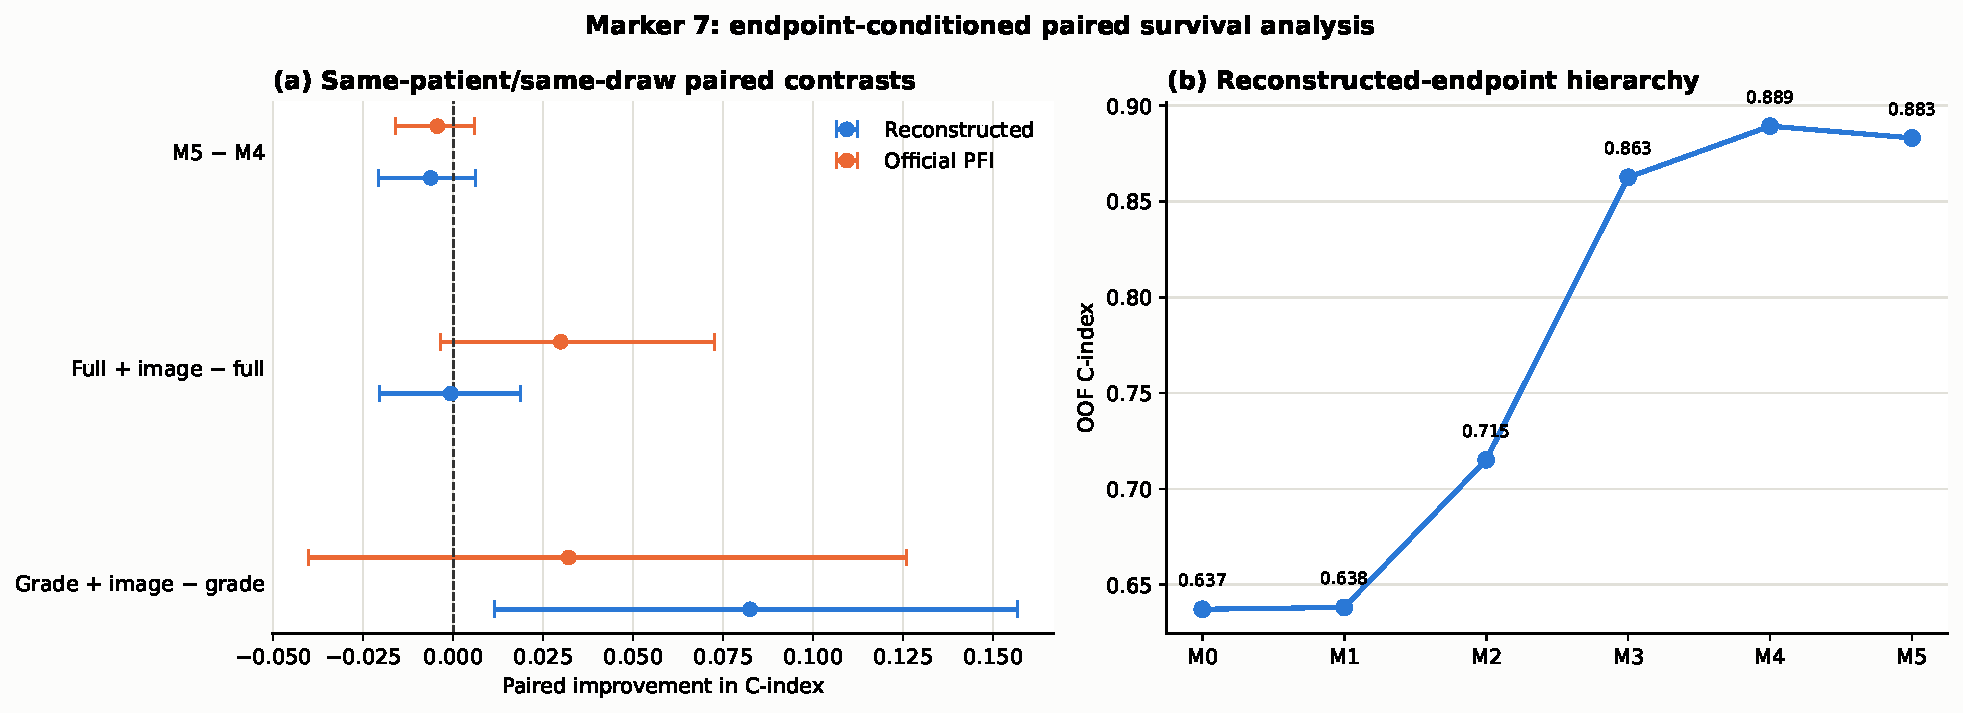
\includegraphics[width=0.95\textwidth]{figures/fig7_marker7_transfer.pdf}
\caption{Historical nested point estimates and clinical-hierarchy context for marker 7. The
finalized comparative interpretation uses the completed same-patient/same-draw R4
common-cohort analysis reported in the text and saved source tables.}
\label{fig:marker7-transfer}
\end{figure}

\subsection{Benchmarking the reconstructed recurrence label against standard TCGA endpoints}
\label{sec:res-label-benchmark}

Because marker 7's TCGA-PRAD label is reconstructed rather than a standard endpoint, we
benchmark it directly against TCGA's own standardized TCGA-CDR endpoints (Liu et al.\ 2018:
progression-free survival, PFS, and disease-free survival, DFS), obtained from cBioPortal study
\texttt{prad\_tcga\_pan\_can\_atlas\_2018}, for the 270-patient embedded cohort. Event-status
agreement is substantial but not perfect: 87.0\% raw agreement with PFS\_STATUS (Cohen's
$\kappa=0.57$, $n=270$) and 93.2\% with DFS\_STATUS (Cohen's $\kappa=0.52$, $n=192$; DFS is
only defined for patients with curative-intent treatment and no prior malignancy, per TCGA-CDR
convention, hence the smaller $n$). Our label flags more patients as having recurred than PFS
does (confusion matrix: 25 patients we label as events that PFS calls censored, vs.\ 10 in the
reverse direction), consistent with our label's coarser, clinical-assessment-based definition
(persistent or recurrent tumor at any follow-up visit) capturing a broader construct than PFS's
progression-specific one. Follow-up time itself agrees closely with both standard endpoints
(Spearman $\rho=+0.85$ vs.\ PFS\_MONTHS, $+0.95$ vs.\ DFS\_MONTHS, both $p<10^{-75}$). A
per-patient provenance table recording every raw follow-up record and the rule used to derive
our label is provided in Supplementary S4.

Official TCGA-CDR progression-free interval (PFI) was mapped one-to-one and evaluably for all
270 frozen-risk patients, with 42 events. Its C-index was 0.586 (95\% patient-bootstrap CI
0.482--0.689; 2{,}000/2{,}000 valid replicates). In this frozen cohort, cBioPortal PFS agreed
exactly with official PFI for event, time, and evaluable population. This cohort-specific exact
agreement does not license treating the endpoint names as interchangeable in general. The
reconstructed endpoint agreed with official PFI for 87.0\% of event indicators
($\kappa=0.57$) and had time Spearman $\rho=0.85$.

Re-scoring marker 7's zero-shot transfer using PFS or DFS directly as the outcome, instead of
our reconstructed label, gives C-index$=0.586$ (td-AUROC@5y$=0.610$, $n=270$, 42 events) against
PFS and C-index$=0.605$ (td-AUROC@5y$=0.592$, $n=192$, only 11 events) against DFS -- both
above chance and directionally consistent with the original C-index$=0.673$ using our
reconstructed label, but visibly attenuated, particularly against PFS's stricter
progression-only definition. We read this as descriptive endpoint sensitivity: the original
C-index$=0.673$ is label-definition-specific, and PFS yields a more modest above-chance
result. The official-PFI result is directionally non-contradictory but not strong support, and
C06 therefore remains bounded to the measured endpoint-specific exploratory evidence.

A stricter endpoint -- requiring a documented tumor-free follow-up visit before a later
with-tumor event, rather than treating any with-tumor observation as recurrence -- changes the
estimand sharply. Of 111 events in all 493 labeled TCGA-PRAD cases, only 11 occur strictly
after an earlier documented tumor-free visit; 100 first/only or same-day with-tumor
observations are reclassified as persistent/indeterminate disease and excluded (Supplementary
S4 gives the full exclusion accounting). Within the embedded cohort this leaves $n=220$ and
only 7 events. Direction is retained (C-index $0.655$, 5-year td-AUROC $0.566$), but seven
events are far too few for a strong recurrence-validation claim. Across the original endpoint,
td-AUROC declines from $0.740$ at 1 year to $0.636$ at 5 years (mean 1--5-year AUC $0.714$,
Figure~\ref{fig:marker7-survival-curves}a), and risk-quintile calibration shows substantial
overprediction (Figure~\ref{fig:marker7-survival-curves}b), consistent with the calibration
slope below one reported above. We therefore characterize marker 7 as an endpoint-sensitive,
post-hoc exploratory transfer. The completed paired analysis above narrows the incremental
interpretation rather than establishing robust independent or incremental prognostic value.

\begin{figure}[htbp]
\centering
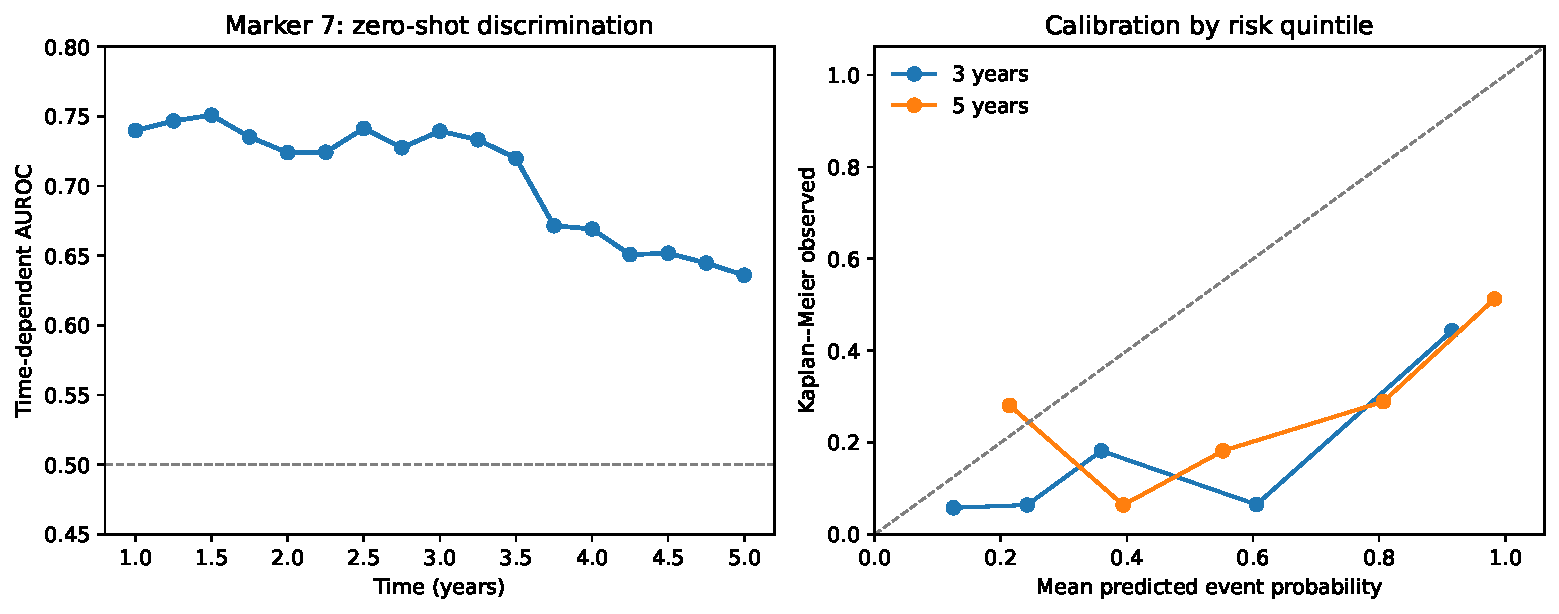
\includegraphics[width=0.90\textwidth]{figures/fig8_marker7_survival_curves.pdf}
\caption{Marker 7 zero-shot survival sensitivity on TCGA-PRAD. Left: time-dependent AUROC
from 1--5 years. Right: predicted vs.\ Kaplan--Meier-observed 3- and 5-year event probability
by predicted-risk quintile. Discrimination remains above chance while absolute risk is
substantially overpredicted without recalibration.}
\label{fig:marker7-survival-curves}
\end{figure}
